\section{Data Analysis}
\label{sec:analysis}

This section provides a detailed analysis of the datasets used in our project, focusing on both curated and web data sources. The goal is to offer a comprehensive overview of the data characteristics.

We begin by presenting statistics for the curated datasets (Section \ref{sec:analysis.curated}), including details on corpus names, languages, text types, and other relevant metadata. We then analyze the web data (Section \ref{sec:analysis.web}), examining the size, composition, and the effects of filtering and deduplication. This includes a breakdown of the number of documents, word counts, and language distributions.

It is important to note how LLM training often uses sampling techniques to optimize data distribution, considering factors like language balance and the fertility score \cite{ali_mehdi_etal_2024}. 
In this paper, we focus solely on the raw data collection, filtering, and integration process, without adjusting distributions for training purposes. For further information on a model trained on part of the data we process, refer to \cite{opengpt_x_2024_13866365}.


\subsection{Curated Data}
\label{sec:analysis.curated}

As previously mentioned, curated data undergoes a distinct processing pipeline. This is due to the assumption that curated datasets generally maintain a higher level of quality, thereby requiring less intensive filtering and deduplication compared to web data. A comprehensive list of the curated datasets used in our study is provided in Table \ref{tab:curated_data_list}, which details 75 datasets, including information on language, format, license, domain, and the number of documents/words, along with the filtering percentage. In the subsequent sections, we will conduct a detailed analysis of the most significant columns.



\begin{figure}
    \centering
    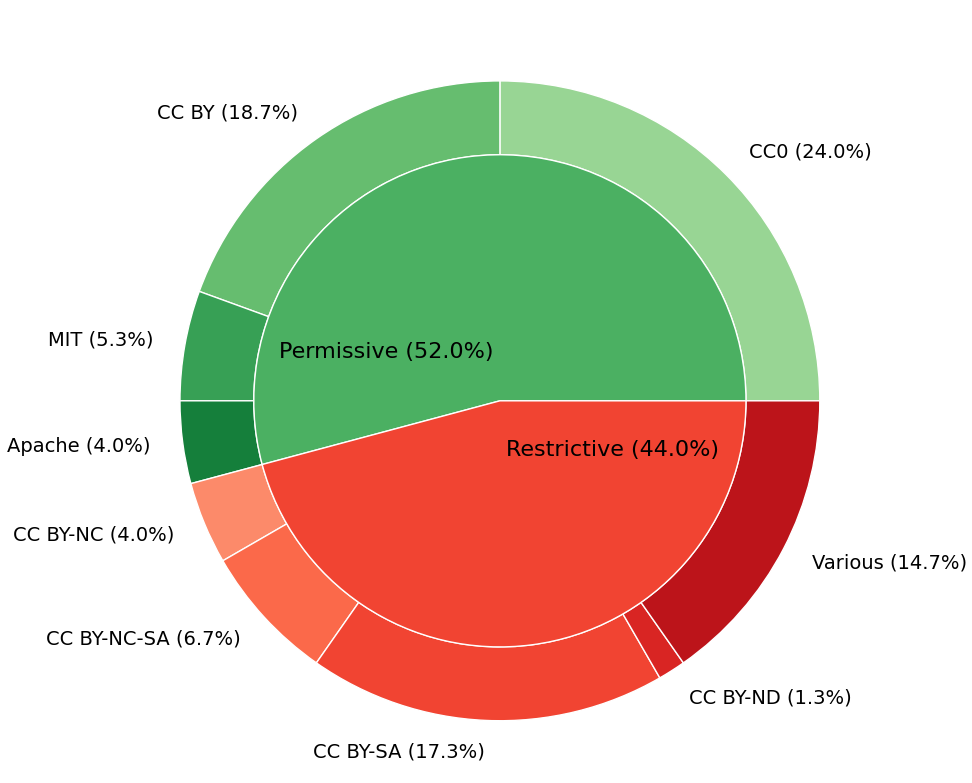
\includegraphics[width=0.6\linewidth]{images/Analysis/licenses.png}
    \caption{\label{fig:licenses}%
    Distribution of curated dataset licenses. Most datasets have permissive licenses (CC0, CC BY, MIT, Apache), 
    while restrictive licenses are primarily represented by datasets sourced from multiple origins (\textit{Various}). }
    
\end{figure}
\subsubsection{Licenses} 
As outlined in the data selection process (see Section \ref{sec:datasets.selection.curated}), selecting datasets according to legal and licensing constraints is a crucial first step. Figure \ref{fig:licenses} illustrates the distribution of licenses across the curated
%%comment: happened as an afterthought, not first step
datasets used in this project. The majority (52\%) of the selected datasets' licenses are permissive and not restricted for commercial use, featuring licenses like CC0 (24\%), CC BY (18.7\%), MIT (5.3\%), and Apache (4\%)\footnote{To simplify aggregation, the license versions are omitted here and in Figure \ref{fig:licenses}. However, in Table \ref{tab:curated_data_list}, the specific version numbers for all the datasets are clearly indicated.}. These licenses enable broad usage of the data, including for commercial purposes, and promote ease of dissemination and integration in various projects.

Conversely, 44\% of the datasets are categorized under restrictive licenses, which limit their use, especially for commercial applications. These include licenses such as CC BY-NC-SA (6.7\%), CC BY-NC (4\%), and the ``Various'' category (14.7\%), which represents datasets compiled from multiple sources and classified under the most restrictive license to mitigate legal risks. 


An important observation is that many datasets did not explicitly mention a license on their official website. For these datasets, we conducted further investigation into the sources, often uncovering related licensing information. However, for some datasets (marked with a dagger in Table \ref{tab:curated_data_list}), we were unable to directly determine the correct licenses despite extensive efforts. 
%In such cases, we made conservative assumptions, classifying them under the license most likely to be applicable based on related materials such as associated code or website. \todo{lennard: Just to be sure, we mean that default copy right laws apply, dont we? Because saying that we assumed the licence could be misleading}


\subsubsection{Languages}
\begin{figure}
\centering
\begin{subfigure}{.5\textwidth}
  \centering
  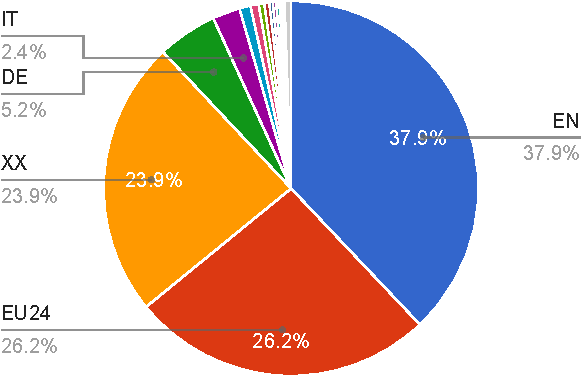
\includegraphics[width=0.95\linewidth]{images/Analysis/curated_lang_words_main.pdf}
  \caption{Complete word distribution} 
  \label{fig:curated_lang_word_a}
\end{subfigure}%
\begin{subfigure}{.5\textwidth}
  \centering
  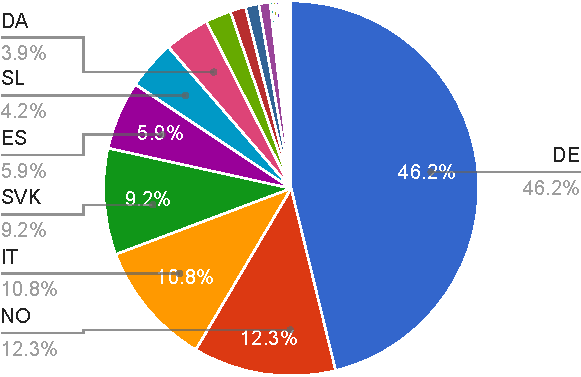
\includegraphics[width=0.95\linewidth]{images/Analysis/curated_lang_words_sub.pdf}
\caption{Word distribution excluding EN, EU24, and XX.}
\label{fig:curated_lang_word_b}
\end{subfigure}
 \caption{Word distribution across different languages in the curated datasets.}
\label{fig:curated_lang_word}
\end{figure}


Our curated dataset encompasses 24 unique languages. For clarity, datasets that include a substantial portion of the official 24 EU languages are grouped under the category “EU24”. Additionally, the analysis also features statistics for other European languages, such as Norwegian (NO). The label “XX” is used to indicate datasets focused on source code.

As shown in Figure \ref{fig:curated_lang_word_a}, English (EN) accounts for 37.9\% of the total word count, followed by the EU24 languages at 26.2\%, and source code (XX) at 23.9\%. Together, these three categories make up 88\% of the curated data. The inclusion of source code is particularly important in this context, as it provides curated, high-quality examples for training models on coding tasks.

Since many datasets feature multiple languages, specific per-language statistics are not always provided, but rather an overall distribution is emphasized.  On average, multilingual datasets contain significantly fewer words (712.8 million) compared to monolingual (4.38 billion) ones. Indeed,  while contributing to language diversity, they often lack the volume of content found in larger monolingual datasets.

After removing the dominant categories (EN, EU24, and XX), Figure \ref{fig:curated_lang_word_b} reveals that German (DE) constitutes 46.2\% of the remaining data. This significant proportion reflects the regional focus of the project, as it is based in Germany, and emphasizes the role of localized datasets in shaping the overall corpus. Other notable languages include Norwegian, Italian, and Spanish, though their contributions remain relatively smaller compared to German.



% Graph values
% Words per language
%EN EU24 XX DE NO IT SK ES SL DA PL FR MA ET BG HR RO HU SK GA EL LT BS MK SQ TR FI
%111512165187.44444 79951548548.0 73064206834.0 10956303105.666666 2920299614.0 2558626263.6666665 2174828161.0 1406434980.5 1007129655.7142857 922700245.0 525519997.71428573 317726618.3333333 276204170.0 227978247.0 61023899.82539683 61023899.82539683 61023899.82539683 53326169.71428572 53326169.71428572 44193174.0 36489045.11111111 23659959.5 7697730.111111111 7697730.111111111 7697730.111111111 7697730.111111111 3650602.0

\paragraph{Analysis of Word Distribution and Dataset Representation in Multilingual Corpora}
One would expect the word distribution to follow the number of datasets available; however, correlation analysis reveals this is only partially true. The Spearman correlation is moderate (0.562, p = 0.0028), while the Pearson correlation indicates a stronger linear relationship (0.855, $P < 0.001$). 
By using linear regression, we observe notable deviations in certain languages. For instance, German (DE) exhibits a significant negative residual, with the actual word count being 5.1 billion fewer than expected, despite having a high number of diverse datasets. This suggests that while German datasets are numerous, they tend to be smaller in size or less word-dense compared to other languages. On the other hand, English (EN) has a positive residual, showing 3.88 billion more words than predicted, which can be attributed to the oversampling of English datasets in the corpus. In contrast, French (FR) underperforms relative to its dataset count, with a negative residual of 1.54 billion, indicating that the French data is underrepresented in terms of word volume.

This analysis underscores the need for balanced sampling across languages. While oversampling English may provide more content for model training, undersampling key languages like French could result in biases that limit the multilingual capabilities of the models. Hence, we recommend strategic oversampling of underrepresented languages and careful moderation of overrepresented languages to ensure linguistic diversity and fairness in the curated dataset.


\subsubsection{Domains}

\begin{table}
\centering
\begin{tabular}{lrrrr}
\hline
Domain                 & \# Datasets & Avg. Words/DS [M] & Total Words [M] & Percentage [\%] \\ \hline
Source Code            & 1        & 73.064                & 73.064      & 40.46           \\
Law and Administration & 22       & 1.674                 & 36.839      & 20.40           \\
Web                    & 6        & 4.120                 & 24.721      & 13.69           \\
Medical                & 5        & 3.229                 & 16.147      & 8.94            \\
Math                   & 6        & 2.684                 & 16.105      & 8.92            \\
Forum                  & 2        & 3.655                 & 7.311       & 4.05            \\
Books                  & 5        & 752                   & 3.763       & 2.08            \\
News                   & 4        & 473                   & 1.893       & 1.05            \\
Knowledge Base         & 4        & 105                   & 423         & 0.23            \\
Culture                & 3        & 48                    & 146         & 0.08            \\
Recreation             & 2        & 73                    & 146         & 0.08            \\ \hline
\end{tabular}
\caption{Total words, average words per dataset (Avg Words/DS), and documents for each domain, sorted by total words. }
\label{tab:word_distribution_per_domain}
\end{table}

The curated dataset spans multiple domains, each contributing a different share to the total word count. Table \ref{tab:word_distribution_per_domain} provides a breakdown of the number of datasets, the average word count per dataset, total word count, and the percentage contribution of each domain.

Source code emerges as the largest domain by word count, accounting for 40.46\% of the total curated data, with over 73 billion words. This is followed by law and administration, which contributes 20.40\%, and the web domain at 13.69\%. Collectively, these three domains represent 74.55\% of the total word count. This strong presence of technical, legal, and digital content suggests that the curated dataset is well-suited for training models focused on tasks related to programming, legal reasoning, and web-based applications.

On the other hand, smaller domains such as culture (0.08\%), recreation (0.08\%), and knowledge base (0.23\%) contribute much less to the overall dataset. These domains are likely underrepresented either due to the limited availability of datasets or their inherently smaller size. 


\subsubsection{Sizes}

The distribution of word counts within the curated dataset is highly skewed, with a few large datasets contributing the majority of the total word volume as shown in Figure \ref{fig:curated_size}. Initially, the largest contributors were \textit{StarCoder}, \textit{EurLex}, and \textit{MaCoCu}, together accounting for 50\% of the total word count. However, since \textit{StarCoder} focuses on source code rather than natural language, it was excluded from further analysis, and the word count distribution was recalculated.

In the revised analysis, four datasets (\textit{peS2o}, \textit{MaCoCu}, \textit{Legal MC4}, and \textit{EurLex}) now make up 50\% of the total word count. Expanding this to 70\%, the dataset contributions broaden to include three additional Pile subsets (\textit{PMC extracts}, \textit{Openwebtext2}, and \textit{Free Law Opinions V2}), as well as \textit{Wikimedia Wikipedia}. Notably, 17 datasets account for 90\% of the total word count, underscoring the significant concentration of data within a limited number of large datasets.

\begin{figure}
    \centering
    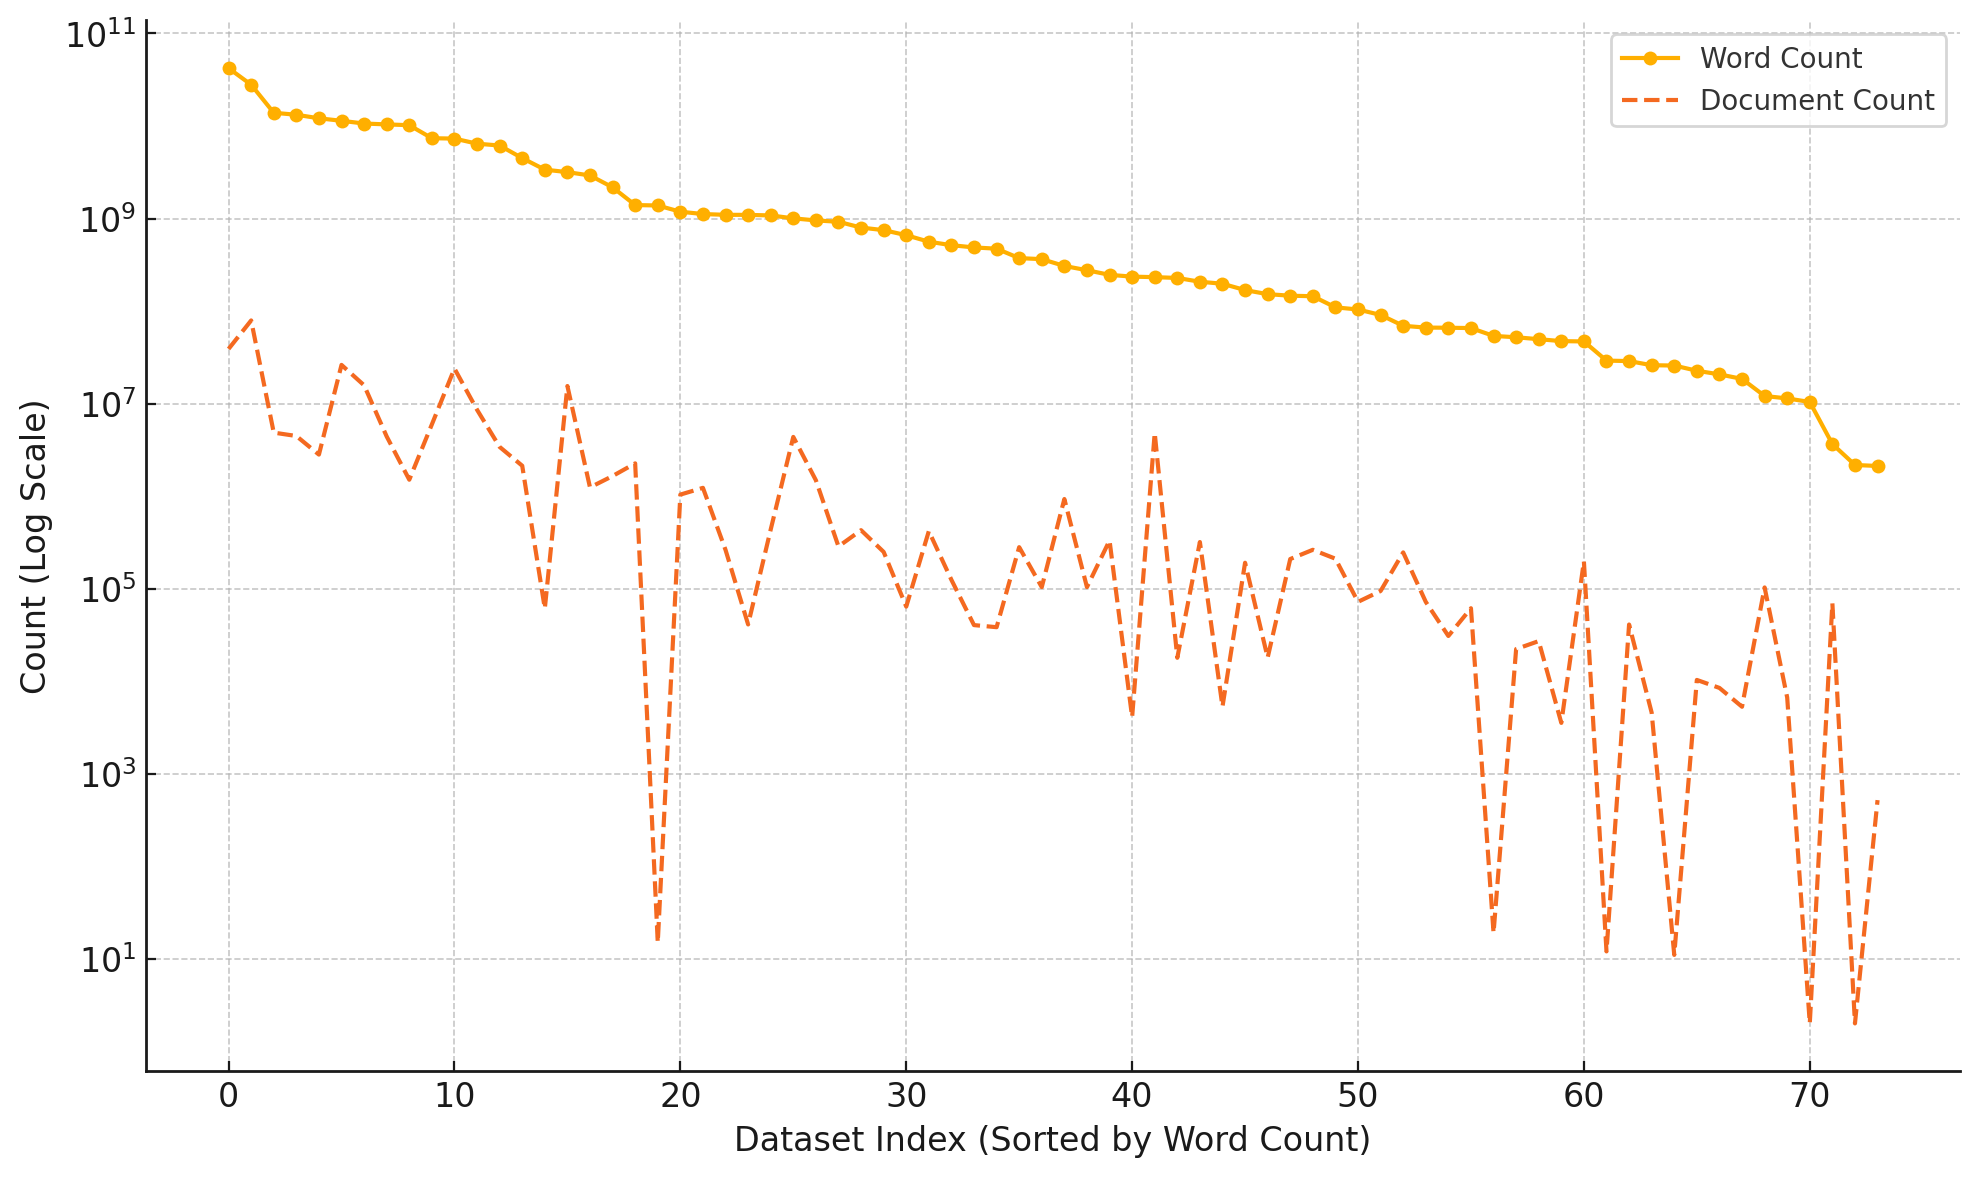
\includegraphics[width=0.7\linewidth]{images/Analysis/curated_size_log.png}
 \caption{Log-scaled comparison of word counts and document counts across datasets, sorted by word size. Some datasets exhibit a notably high word count despite having relatively few documents, indicating longer average document sizes.}    \label{fig:curated_size}
\end{figure}

Additionally, certain datasets display an unusually high word count relative to their document counts. A regression analysis was performed to better understand these discrepancies, calculating residuals to detect significant deviations from the expected document-to-word ratio. This analysis revealed the following outliers:

\begin{itemize} 
\item \textit{Spanish legal corpora (ES)}: This legal corpus consists of only 15 documents but contains over 1.38 billion words. The residual analysis (5.4) shows that the word count is approximately 221 times higher than expected based on the number of documents. This suggests that individual documents within this corpus are unusually large.

\item \textit{Projekt Gutenberg (EU24)}: A well-known collection of books, \textit{Projekt Gutenberg} contributes over 3.37 billion words with only 60,912 documents. This results in a positive residual of 1.8, indicating that the dataset's word count per document is significantly higher than the regression model predicted. This observation aligns with expectations for book collections, as books typically contain more words per document compared to other formats such as articles or reports.

\item \textit{Pile: PMC extracts (EN)}: A medical dataset with 2.8 million documents and over 12.1 billion words, \textit{PMC extracts} exhibits a positive residual of 1.07. This indicates that the word count is significantly higher than predicted by the model. This is expected, as the dataset primarily contains full-length medical research articles, which are generally more detailed and content-rich compared to other document types.

\end{itemize}


\subsubsection{Filtering}

Across the curated datasets, the average filtering percentage is 5.33\% ($\pm 5.98\%$). Based on these values, filtering can be  split in three categories:

\begin{itemize}
    \item Low Filtering ($<1\%$): Datasets that underwent minimal filtering, typically because they contained well-structured, clean data to begin with. 
    
    \item  Medium Filtering (1\% to 11.31\%): The majority of datasets fall into this category, with moderate filtering applied to remove noise or short documents without heavily impacting the total word count. 
    
    \item  High Filtering (>11.31\%): Datasets with a high filtering percentage, indicating substantial noise or irrelevant content. 
\end{itemize}

In reviewing the impact of filtering, we found that documents with low language scores typically fall into one of four categories: i) mixed-language documents, ii) documents with conversion errors containing numerous special characters, iii) documents involving closely related languages (e.g., Croatian and Serbo-Croatian), and iv) documents in low-resourced languages where the content was misidentified as a different language. 

To further understand the impact of filtering across datasets, we explored potential correlations between the percentage of filtered data and several key dataset characteristics: the number of words, number of documents, format, language, and domain. Our analysis showed only modest correlations in most cases, indicating that filtering tends to act somewhat independently of these factors (refer to Appendix \ref{sec:appendix.curated.filtering} for a more detailed analysis).


\subsubsection{Summary}
The curated dataset presents a comprehensive and diverse collection of 75 datasets spanning 25 languages, various domains, and multiple formats, offering a robust foundation for a wide range of research tasks. Despite some imbalances in distribution, particularly with large datasets dominating the total word count, the variety within the dataset makes it a valuable asset for training LLMs. The high presence of technical and legal data, alongside source code, reflects the strengths of this dataset in supporting tasks in these fields.

While filtering in general is necessary to ensure data quality, its impact on the curated datasets is relatively moderate, with only a few datasets requiring significant cleaning. The weak correlations found between filtering percentages and dataset characteristics suggest that filtering is driven more by the specificities of the dataset than by its size, format, or domain. 
In preparing data for training LLMs, we found that a strategic approach to selecting subsets is key. Leveraging the wide domain and language diversity can help ensure more balanced outcomes. 

%\href{https://fraunhofer-my.sharepoint.com/:x:/r/personal/johannes_leveling_iais_fraunhofer_de/_layouts/15/Doc.aspx?sourcedoc=%7BD7ADD271-ED4B-47CA-86F5-CE62A599F912%7D&file=llm_corpora.xlsx&wdLOR=c27B8055B-BD02-B442-B99A-3F6FD43B68A0&fromShare=true&action=default&mobileredirect=true}{ap2}
%\href{https://fraunhofer-my.sharepoint.com/:x:/g/personal/michael_fromm_iais_fraunhofer_de/EcT21_OK0phDnM7qnC2VBQwBv3x4c5B4KO6Fm9Mum4xAmw?e=oRAZZp&wdOrigin=TEAMS-MAGLEV.p2p_ns.rwc&wdExp=TEAMS-TREATMENT&wdhostclicktime=1724229183141&web=1}{ap3}

% \href{https://fraunhofer-my.sharepoint.com/:w:/g/personal/ines_wendler_iais_fraunhofer_de/EYbxNGHzv0tNmgNe3ay1Ty8Bho28_6Px8HdK2K8yhayblg?e=rwf8MA&wdOrigin=TEAMS-MAGLEV.p2p_ns.rwc&wdExp=TEAMS-TREATMENT&wdhostclicktime=1724241908075&web=1}{legal contract}

 
\subsection{Web Data}
\label{sec:analysis.web}
%
% https://fraunhofer-my.sharepoint.com/:x:/g/personal/ines_wendler_iais_fraunhofer_de/EVj7bq4zU4dKt-E6fAE6xPgBK-Z3C80nx4qAfFi9P0gjfw?e=HAxml7&wdOrigin=TEAMS-MAGLEV.p2p_ns.rwc&wdExp=TEAMS-TREATMENT&wdhostclicktime=1712751229207&web=1

% Pavel: this information is from the Ines spreadsheet (link above), the numbers are very different from what Michael provided
We source the web data from the Common Crawl dumps released between 2014 and 2023.
The filtering step keeps about 14\% of the documents from the Ungoliant output.
The deduplication step keeps about 86\% of the documents from the filtering step, or about 12\% of the documents from the Ungoliant output.
The final 3.4 billion documents contain about 30 trillion words in total, or 8000 words per document on average.

% 1. AP2 attempt of data catalog for web data https://fraunhofer-my.sharepoint.com/:x:/r/personal/nicolo_brandizzi_iais_fraunhofer_de/_layouts/15/Doc.aspx?sourcedoc=%7BBE579811-082D-4901-946A-4F864B954CB9%7D&file=FhG%20Data.xlsm&action=default&mobileredirect=true

% 2. AP3 excel for training phases 
%https://fraunhofer-my.sharepoint.com/:x:/r/personal/michael_fromm_iais_fraunhofer_de/_layouts/15/Doc.aspx?sourcedoc=%7BFFD598FC-27BE-4AC3-BF70-7FBF7BF844A0%7D&file=OpenGPT-X-7B-Training.xlsx&action=default&mobileredirect=true

% 3. AP3 link with oscar info based on focus on 4 langauges 
%https://fraunhofer-my.sharepoint.com/:x:/r/personal/michael_fromm_iais_fraunhofer_de/_layouts/15/Doc.aspx?sourcedoc=%7BF3D7F6C4-D28A-4398-9CCE-EA9C2D95050C%7D&file=OpenGPT-X%20Phase%201.xlsx&action=default&mobileredirect=true

% dump used with number of pages/docs in billion . Need to find how many tokens per page
% This data comes from here :https://fraunhofer-my.sharepoint.com/:x:/g/personal/ines_wendler_iais_fraunhofer_de/EVj7bq4zU4dKt-E6fAE6xPgBK-Z3C80nx4qAfFi9P0gjfw?e=HAxml7&wdOrigin=TEAMS-MAGLEV.p2p_ns.rwc&wdExp=TEAMS-TREATMENT&wdhostclicktime=1712751229207&web=1
% which is the billion pages per dump reported by commoncrawl cross referenced with ap3 link (#3)
% {'2014-42': 3.72, '2015-14': 1.64, '2015-48': 1.82, '2016-22': 1.46, '2016-44': 3.25, '2017-13': 3.07, '2017-47': 3.2, '2018-30': 3.25, '2018-47': 2.6, '2019-22': 2.65, '2020-24': 2.75, '2020-45': 2.71, '2021-31': 3.15, '2021-49': 2.5, '2022-27': 3.1, '2022-40': 3.15, '2022-49': 3.35, '2023-06': 3.35, '2023-14': 3.1, '2023-23': 3.1, '2017-51': 2.9, '2018-05': 3.4, '2018-09': 3.4, '2018-13': 3.2, '2018-17': 3.1, '2018-22': 2.75, '2018-26': 3.05, '2018-34': 2.65, '2018-39': 2.8, '2018-43': 3.0, '2018-51': 3.1, '2019-04': 2.85, '2019-09': 2.9, '2019-13': 2.55, '2019-18': 2.5, '2019-26': 2.6, '2019-30': 2.6, '2019-35': 2.95, '2019-39': 2.55, '2019-47': 2.55, '2019-51': 2.45, '2020-05': 3.1, '2020-10': 2.6, '2020-16': 2.85, '2020-29': 3.14, '2020-34': 2.45, '2020-40': 3.45, '2020-50': 2.64, '2021-04': 3.4, '2021-10': 2.7, '2021-17': 3.1, '2021-21': 2.6, '2021-25': 2.45, '2021-39': 2.95, '2021-43': 3.3, '2022-05': 2.95, '2022-21': 3.45, '2022-33': 2.55, '2023-40': 3.4, '2023-50': 3.35}

%60 dumps where used with the earliest being 2014-42 and the latest 2023-5 with A total of 173 billion documents 

As previously mentioned (Section \ref{sec:datasets.selection.cc}), the web data used in this project was sourced from CommonCrawl. For this study, we utilized 60 distinct dumps from CommonCrawl, spanning a broad timeframe. The earliest dump was week 42 of 2014 (2014-42), and the most recent dump was week 5 of 2023 (2023-5). This extensive range allowed us to capture a wide variety of web content across nearly a decade, ensuring that the dataset reflects both historical and contemporary web information.

On average, each CommonCrawl dump contains approximately 2.7 billion documents. Across all 60 dumps, we accumulated a total of 173 billion documents, representing around 703 terabytes of raw, unprocessed data. This vast volume of data provided a strong foundation for training large-scale language models but also introduced significant challenges in terms of data processing and filtering, as discussed in previous sections.


\begin{table}[htb!]
\centering
\begin{tabular}{cl}
\toprule
\textbf{Year} & \textbf{Week} \\ 
\midrule
2014         & 42               \\ 
2015         & 14, 48           \\ 
2016         & 22, 44           \\ 
2017         & 13, 47, 51       \\ 
2018         & 5, 9, 13, 17, 22, 26, 30, 34, 39, 43, 47, 51 \\ 
2019         & 4, 9, 13, 18, 22, 26, 30, 35, 39, 47, 51 \\ 
2020         & 5, 10, 16, 24, 29, 34, 40, 45, 50 \\ 
2021         & 4, 10, 17, 21, 25, 31, 39, 43, 49 \\ 
2022         & 5, 21, 27, 33, 40, 49 \\ 
2023         & 6, 14, 23, 40, 50 \\ 
\bottomrule
\end{tabular}
\caption{List of dumps by year and week.}
\label{tab:dumps_by_year}
\end{table}


\paragraph{Dumps}
In this section, we provide a detailed look at the CommonCrawl dumps used in our project. The dumps span multiple years, with varying distributions of weeks per year. Table \ref{tab:dumps_by_year} presents  the list of years and the corresponding weeks for each dump.

% Julich
% 2014: 42 (done)
% 2015: 14 (done), 48 (done)
% 2016: 22,(ongoing) 
% 2017: 13(ongoing), 47(done), 51(done)
% 2018: 05 , 09, 13, 17, 22, 26, 30, 34, 39, 43, 
% 2019: 51
% 2020: 05, 10,16, 29, 34, 40, 50
% 2021: 04, 31
% 2022: 27, 40, 
% 2023: 06, 14, 23, 

% Dresden
% 2014:
% 2015:
% 2016:
% (2018): 47, 51
% 2019: 04, 09, 13, 18, 22, 26, 30 , 35, 39,  47
% (2020): 24, 45
% (2021): 10, 17, 21, 25, 39, 43, 49
% (2022): 05, 21, 33, 49, 
% 2023: 40, 50

% Missing
% 2014:
% 2015:
% 2016: 44
% 2018: 
% 2019: 51
% 2020:
% 2021: 
% 2022: 
% 2023:



As can be seen from the list, the distribution of dumps across weeks is uneven. Earlier years, particularly 2014 through 2016, have fewer weeks represented compared to more recent years. However, the dumps from these earlier years typically contain a higher dump density, i.e. average document size (see Figure \ref{fig:dumps_distribution}). After 2017, CommonCrawl transitioned to a strategy of producing more frequent dumps, each with relatively smaller average document sizes.

This shift in strategy has important implications for data processing. Special attention must be paid to the earlier years (2014–2016), where deduplication can be more computationally expensive due to the larger document sizes. In these cases, employing stricter filtering mechanisms may be necessary to ensure efficient processing and to avoid excessive resource consumption during deduplication.


% DATA for graphs
% years 2014 2015 2016 2017 2018 2019 2020 2021 2022 2023
% len(year) 1 2 2 3 12 11 9 9 6 5
% size(year) 22.53 17.98 16.91 37.28 36.3 32.15 25.69 26.15 18.55 16.3
% avg(size(year)) 22.53 8.99 8.455 12.426 2.025 2.922 2.854 2.905 3.091 3.260





\begin{figure}
\centering
  \centering
  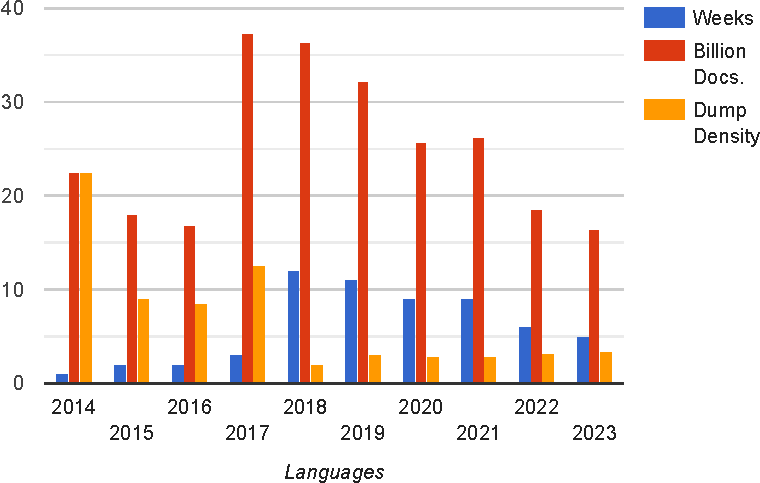
\includegraphics[width=0.75\linewidth]{images/Analysis/docs_weeks_density_xyear.pdf}
\caption{Analysis of CommonCrawl dumps used in the dataset, showing the distribution of dump weeks (blue), billion documents (red) and average dump density (yellow) per year.}
\label{fig:dumps_distribution}
\end{figure}



\paragraph{Compute power}

% For these numbers i used benny's 'dedup_cpu_requirements.html'. Specifically, step 2, old estimate. I tool the total for en 210, computed the percentage going in dedup and filtering. Used that percentage on the total estimated BEFORE code (504k), divided by 110 to get the "per dump" and then tiems 60 to get the total 
Tracking the compute power required during data processing is essential for planning and securing the necessary resources. A well-structured plan not only ensures that adequate resources are available but also provides an opportunity to analyze computational efficiency and sustainability.

Below, we estimated total CPU hours consumed at each stage of the pipeline:

% \todo[inline]{BS: I don't know how you got those numbers? (Perhaps it would also be interesting for the reader - if it is not too complicated to explain\dots NB: fill out footnote) }

\begin{itemize}
    \item Conversion: On average, converting a dump takes 115,2 CPU hours. For all the data combined this stage took 6,912 CPU hours.
    \item Filtering: On average, filtering one dump takes 763 CPU hours. For all dumps combined, this stage required 45,810 CPU hours. 
    \item Deduplication: Deduplication is notably resource-intensive, taking an average of 3,680 CPU hours per dump. For the entire dataset, this stage consumed 221,230 CPU hours. 
\end{itemize}


Deduplication is by far the most time-consuming step, consuming 80.8\% of the total compute power, which is why it is kept as the final stage in our pipeline (see Section \ref{sec:pipelines.web.dedup}). This is followed by filtering, which takes 16.7\%, and conversion, accounting for 2.5\%.


% \paragraph{Filtering effect}
% \todo{NB: todo}


\paragraph{Deduplication Effect}

\begin{figure}
  \centering
  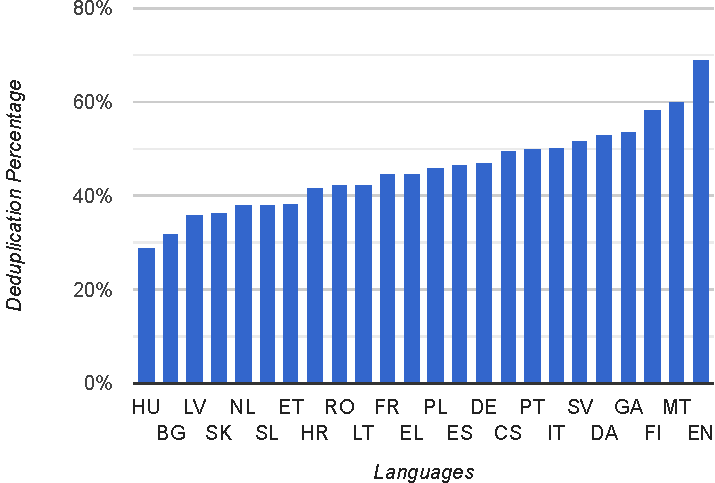
\includegraphics[width=0.7\linewidth]{images/Analysis/dedup_perc_lang.pdf}
  \caption{ Percentage of data removed after deduplication for each language, showcasing the varying impact of deduplication.} 
  \label{fig:dedup_perc_lang}
\end{figure}


% Data from link #2 showing percentage of dedup data for each language taken from tab 'phase 1'
%HU BG LV SK NL SL ET HR RO LT FR EL PL ES DE CS PT IT SV DA GA FI MT EN
% 0.2903 0.31920000000000004 0.35969999999999996 0.3635 0.38 0.3812 0.3825 0.4164 0.4218 0.4235 0.4458 0.44630000000000003 0.46049999999999996 0.4656 0.46840000000000004 0.4953 0.4996 0.5047 0.5156000000000001 0.5301 0.537 0.5827 0.5993999999999999 0.6895

Our deduplication methodology is based on a MinHash + Locality Sensitive Hashing approach that is explained in detail in \cite{leveling_helmer_etal2024}, where the choice of algorithm, along with precision and recall metrics, are analyzed. 
In this section, we shift focus to examining how deduplication disproportionately affects different languages. Figure \ref{fig:dedup_perc_lang} illustrates the percentage of data removed after deduplication for each language, ranging from a minimum of 29.03\% for Hungarian to a maximum of 68.95\% for English. While it may seem intuitive to correlate the deduplication percentage with data availability, a Pearson correlation analysis reveals only a modest positive correlation of 0.54 (p = 0.006).

This suggests that some languages may be subject to an ``unfair'' amount of deduplication relative to their size. Although deduplication operates by identifying and removing similar content, this implies that certain languages contain a higher proportion of similar data, which may result in a final model that struggles to capture linguistic nuances.


To evaluate this disproportionality, we introduce the \textit{Deduplication Disparity Index} (DDI), which measures the impact of deduplication on each language relative to its available web data. For each language \( l \), the DDI is calculated as the Z-score of the deduplication-to-data ratio \( R_l \), which measures the percentage of data deduplicated in relation to the total web data available for that language:


\[
\operatorname{DDI}_l = \frac{R_l - \mu_R}{\sigma_R}, \quad \text{where} \quad R_l = \frac{d_l}{W_l}
\]



Here, \( d_l \) is the deduplication percentage for language \( l \), \( W_l \) is the total number of web data words for language \( l \), \( \mu_R \) is the average deduplication-to-data ratio across all languages, and \( \sigma_R \) is the standard deviation of the deduplication-to-data ratios. This Z-score transformation centers the $\operatorname{DDI}$ around zero, highlighting languages where deduplication has a disproportionately high or low impact.

Languages with a high positive Z-score, such as Maltese ($\operatorname{DDI}_{mt}=4.519$) and Croatian ($\operatorname{DDI}_{mt}=1.0735$), are significantly impacted by deduplication, while others have scores closer to zero ($\operatorname{DDI} = -0.25 \pm 0.012)$, indicating a more balanced deduplication-to-data ratio. This metric provides a systematic way to assess fairness in the data processing pipeline and highlights languages that might require further attention during preprocessing.

% \todo[inline]{BS: Are the DDIs shown somewhere in a table or diagram? NB: no, i think we have enough tables already, maybe in revised }

\subsubsection{Summary} 
The web data for this project was sourced from 60 distinct CommonCrawl dumps spanning 2014 2023, resulting in a total of 173 billion documents (703 terabytes of raw data). This broad timeframe captures both historical and contemporary web content.

Deduplication was the most resource-intensive step, consuming 80.8\% of total CPU hours allocated for data processing. We introduced the Deduplication Disparity Index (DDI) to identify languages disproportionately affected by deduplication, highlighting the need for tailored processing strategies to ensure fairness and data quality. 



